\documentclass[UTF8]{ctexart}
\usepackage{amsmath}
\usepackage{mathtools}
\usepackage{geometry}
\usepackage{cases}
\usepackage{tikz}
\usepackage{enumitem}
\usepackage{graphicx}
\usepackage{float}
\setlength{\parindent}{0pt}
\geometry{a4paper,scale=0.73}
\title{每日一题(5.1)答案}
\author{选题:门宇翎、李东宸\\答案制作:程昊一}

\begin{document}
\maketitle

\hspace*{2em}\textbf{1.}{\CJKfamily{kai}若$n$为正整数,且$2^n-1$为素数,证明:$n$也为素数.\\(门宇翎供题)}\\
\hspace*{2em}\textbf{分析}\quad 我们要证明$n$为素数,一种最暴力的方法是枚举所有的$n$,然后逐个验证,但在这道题中显然是行不通的.还有一种办法,我们利用\textbf{反证法},假设$n$为合数,导数矛盾,证明了$n$为素数.\\
\hspace*{2em}\textbf{解}\quad 若$n$不为素数,则一定存在\textbf{不为1}的$n_1,n_2$,使得$n=n_1\cdot n_2$.则
\begin{align*}
2^n-1&=2^{n_1\cdot n_2}-1\\
&=\left(2^{n_1}\right)^{n_2}-1\\
&=(2^{n_1}-1)[\left(2^{n_1}\right)^{n_2-1}+\left(2^{n_1}\right)^{n_2-2}+\dots+2^{n_1}+1]
\end{align*}
我们在这里把$2^n-1$分解为两个大于1的数的乘积,所以$2^n-1$为合数,与题目矛盾!\\
\hspace*{2em}所以假设不成立,原命题成立.\\
\hspace*{2em}\textbf{注}\quad 我们利用了一个公式:
\[a^n-1=(a-1)(a^{-1}+a^{n-2}+\dots+a+1)\]
更一般地:
\[a^n-b^n=(a-b)(a^{n-1}+a^{n-2}b+a^{n-3}b^2+\dots+ab^{n-2}+b^{n-1})\]

\hspace*{2em}\textbf{2.}{\CJKfamily{kai}如图,两个同心圆构成的圆环被均匀分割成7份,联通中间的校园共8个区域.若要给这8个区域着色,至少要用几种颜色,才能使相邻区域染不同的颜色?\\(李东宸供题)}\\
\begin{figure}[H]
\centering
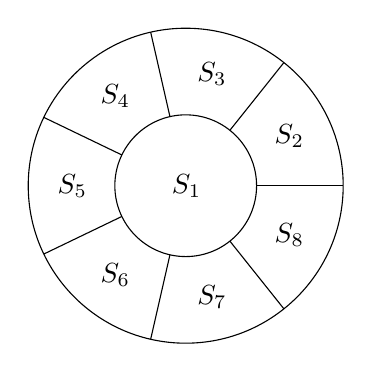
\begin{tikzpicture}
	\draw (0,0) circle(0.9);
	\node at (-0.3,0) [right]{$S_1$};
	\draw (0,0) circle(2);
	\foreach \x in {0,1,2,3,4,5,6}
		\draw [rotate={51.42857 * \x}] (0.9,0)--(2,0);
	\node at (1.0064,0.6291)[right]{$S_2$};
	\node at (0.0227,1.4136)[right]{$S_3$};
	\node at (-1.2041,1.1336)[right]{$S_4$};
	\node at (-1.75,0)[right]{$S_5$};
	\node at (-1.2041,-1.1337)[right]{$S_6$};
	\node at (0.0227,-1.4136)[right]{$S_7$};
	\node at (1.0064,-0.6291)[right]{$S_8$};
\end{tikzpicture}

\end{figure}

\hspace*{2em}\textbf{解}\quad 将8个区域分别记为$S_1,S_2,\dots,S_8$.不妨设$S_1$为红色.则$S_2,S_3,\dots,S_8$都不为红色.\\
\hspace*{2em}如果$S_2,S_3,\dots,S_8$中只有两种颜色,设为黄色和蓝色.我们不妨设$S_2$为黄色.则$S_3$为蓝色.所以,$S_4$为黄色,$\dots,S_7$为蓝色.这时我们发现,无论$S_8$是黄色还是蓝色,都会导致矛盾.所以,$S_2,S_3,\dots,S_8$中不能只有两种颜色.\\
\hspace*{2em}所以,$S_2,S_3,\dots,S_8$中至少有三种颜色,连同$S_1$,共4种颜色.构造如下:
\begin{figure}[!ht]
\centering
\includegraphics[width=7cm]{example.jpg}
\end{figure}

\end{document}